%% Copernicus Publications Manuscript Preparation Template for LaTeX Submissions
%% ---------------------------------
%% This template should be used for copernicus.cls
%% The class file and some style files are bundled in the Copernicus Latex Package, which can be downloaded from the different journal webpages.
%% For further assistance please contact Copernicus Publications at: production@copernicus.org
%% https://publications.copernicus.org/for_authors/manuscript_preparation.html

%% Please use the following documentclass and journal abbreviations for preprints and final revised papers.

%% 2-column papers and preprints
\documentclass[hess, manuscript]{copernicus}

%% Journal abbreviations (please use the same for preprints and final revised papers)
% Hydrology and Earth System Sciences (hess)

%% \usepackage commands included in the copernicus.cls:
%\usepackage[german, english]{babel}
%\usepackage{tabularx}
%\usepackage{cancel}
%\usepackage{multirow}
%\usepackage{supertabular}
%\usepackage{algorithmic}
%\usepackage{algorithm}
%\usepackage{amsthm}
%\usepackage{float}
%\usepackage{subfig}
%\usepackage{rotating}
\usepackage{textcomp} % use %
\usepackage{hyperref} % use hyperlinks
\hypersetup{colorlinks=true, citecolor=blue}


\begin{document}

\title{Climate and Cryosphere Cause Regime Shifts in Water Yield over the Upper Brahmaputra River}

% \Author[affil]{given_name}{surname}
\Author[1]{Hao}{Li}
\Author[2]{Liu}{Liu}
\Author[3]{Baoying}{Shan}
\Author[4]{Lei}{Wang}
\Author[1]{Akash}{Koppa}
\Author[5]{Feng}{Zhong}
\Author[6]{Dongfeng}{Li}
\Author[2]{Xuanxuan}{Wang}
\Author[2]{Wenfeng}{Liu}
\Author[7]{Zongxue}{Xu}

\affil[1]{Hydro-Climate Extremes Lab, Ghent University, Ghent, Belgium}
\affil[2]{Center for Agricultural Water Research in China, China Agricultural University, Beijing, China}
\affil[3]{Research Unit Knowledge-based Systems, Ghent University, Ghent, Belgium}
\affil[4]{Institute of Tibetan Plateau Research, Chinese Academy of China, Beijing, China}
\affil[5]{College of Hydrology and Water Resources, Hohai University, Nanjing, China}
\affil[6]{Department of Geography, National University of Singapore, Singapore}
\affil[7]{College of Water Sciences, Beijing Normal University, Beijing, China}

%% The [] brackets identify the author with the corresponding affiliation. 1, 2, 3, etc. should be inserted.
%% If an author is deceased, please mark the respective author name(s) with a dagger, e.g. "\Author[2,$\dag$]{Anton}{Smith}", and add a further "\affil[$\dag$]{deceased, 1 July 2019}".
%% If authors contributed equally, please mark the respective author names with an asterisk, e.g. "\Author[2,*]{Anton}{Smith}" and "\Author[3,*]{Bradley}{Miller}" and add a further affiliation: "\affil[*]{These authors contributed equally to this work.}".

\correspondence{Liu Liu (liuliu@cau.edu.cn)}

% These dates will be inserted by Copernicus Publications during the typesetting process.
\runningtitle{TEXT}
\runningauthor{TEXT}

\received{}
\pubdiscuss{} %% only important for two-stage journals
\revised{}
\accepted{}
\published{}
\firstpage{1}

\maketitle

\begin{abstract}
Although evidence of hydrological responses to climate is abundant, changes in water yield (WY) in mountainous regions due to climate change and intensified cryospheric melt remain unclear, mainly because of limited observations and large uncertainties in cryosphere-hydrological modeling. 
In this study, we used annual runoff observations and a high-resolution precipitation dataset to examine the long-term changes in WY in the Upper Brahmaputra River (UBR) basin, as represented by six sub-basins from the stream head to downstream. 
We found that WY generally increased during 1982--2013, but regime shifts were detected in the late 1990s. Moreover, the direction of the changes in WY reversed from increasing to decreasing in recent years despite the magnitude of the changes continually increasing from less than 10\% to 80.5\%. 
Furthermore, we used the double mass curve technique to assess the effects of climate, vegetation, and the cryosphere on WY. The results showed that the climate and cryosphere together contributed to over 80\% of the magnitude increases in WY over the entire UBR basin. 
However, the combined effects were either offsetting or additive, further leading to slight or substantial magnitude increases, respectively, in which the role of vegetation was nearly negligible. 
Nevertheless, we found that meltwater from the cryosphere had the potential to alleviate the loss of water availability, which mainly resulted from reduced effective precipitation in most regions. Therefore, the combined effects of climate and cryosphere changes should be considered in ecological restoration and water resources management, particularly involving co-benefits for upstream and downstream regions.
\end{abstract}


\introduction
Water yield (WY) in mountains is crucial for sustaining fragile ecosystems in the headwaters, supplying valuable freshwater resources to downstream lowlands, and balancing co-benefits between the upstream and downstream areas, especially for large transboundary river systems \citep{viviroli2011climate}. 
In mountainous regions, changes in WY have been commonly, but separately, attributed to climate changes \citep{dierauer2018climate,song2021river}, vegetation \citep{goulden2014mountain,zhou2021divergent}, and the cryosphere (such as glacial snow melt; see \citealt{kraaijenbrink2021climate}). 
These changes are expected to alter the spatial and temporal distribution of water resources \citep{tang2019streamflow} and further threaten the water supply and food security downstream \citep{biemans2019importance}.
Despite some in situ observations and runoff estimates from state-of-the-art remote sensing technology, the total river runoff for the Third Pole, which is also known as the “Asian Water Tower,” has never been reliably quantified, and its responses to climate change remain unclear \citep{wang2021tp}. 
Therefore, comprehensively assessing the impacts of the climate, vegetation, and cryosphere on long-term changes, particularly in magnitude and direction, in WY in this region is of great importance for the sustainable development of water resources and ecological environment \citep{yao2019recent}. 

The Qinghai-Tibet Plateau (QTP), regarded as the center of the Third Pole, is one of the most sensitive and vulnerable mountainous regions to environmental changes \citep{kang2010review,yao2010glacial,yao2019recent} and supplies water resources for major rivers in Asia, such as Brahmaputra, Salween, Mekong, Yangtze, Yellow, and Indus Rivers. 
Changes in WY in this region are a crucial factor in the use of water resources, prevention of natural disasters, and protection of aquatic functions for the livelihoods of approximately two billion people in the area \citep{immerzeel2010climate}. In recent years, changes in the climate, vegetation, and cryosphere have significantly affected the WY over the QTP \citep{bibi2018climatic}. 
For example, \citet{fan2015temperature} highlighted the effects of precipitation on the direction of change in WY over the Salween and Mekong River basins. \citet{li2020substantial} determined that elevated precipitation and warming-induced changes in glacial snow patterns both contributed to the magnitude of the increase in WY for the Tuotuo River (a headwater of the Yangtze River). Similarly, \citet{lutz2014consistent} projected that increased precipitation near the Salween and Mekong Rivers and accelerated meltwater near the Indus River caused major changes  in WY. 
Moreover, the role of vegetation in mountain water resources is important. \citet{li2017grassland} showed that increased evapotranspiration, mostly due to grassland restoration, decreased the WY in the Yangtze River basin, while \citet{li2021vegetation} suggested that vegetation greening was mainly linked to the positive WY trend during the dry season over the Brahmaputra River. 

Although a growing body of evidence has shown that WY is affected by climate, vegetation, and cryosphere in the QTP, most studies have focused on individual sub-basins and have not considered these three aspects together throughout this large and understudied region \citep{dierauer2018climate, goulden2014mountain,kraaijenbrink2021climate, song2021river,zhou2021divergent}. 
Therefore, previous results may not fully reveal the spatial variability in the region. Of specific interest is the Upper Brahmaputra River (UBR) basin, which covers an area of over 198,636 km$^2$ (Table S1) and has large gradients in elevation, climate, and vegetation \citep{li2019spatiotemporal}.
Therefore, providing a comprehensive, spatially differentiated study of the WY changes in the UBR basin that considers the joint effects of the climate, vegetation, and cryosphere is imperative. However, studies of WY changes in this region are significantly hindered by the sparse network of hydrological observation stations \citep{li2019spatiotemporal,wang2021tp,yao2019recent}, which leads to large uncertainties in WY forecasts and, thus, water resources assessments.
In addition, current precipitation estimates are highly uncertain owing to the complex topography of the region, which limits the ability to accurately model the relationships between precipitation and runoff \citep{sun2020precipitation}. 
Lastly, the present limited understanding of WY responses to the joint interaction of the climate, vegetation, and cryosphere has become the biggest challenge for developing accurate physically-based cryosphere-hydrological models \citep{pellicciotti2012challenges}. Nevertheless, long-term runoff data and high-resolution satellite records of climate and vegetation cover provide a potential pathway for determining their relationships using statistical 

In this study, we collected annual runoff data for 1982--2013 from six hydrological stations to detect long-term changes in the WY over the UBR basin. In addition, a modified double mass curve (DMC) method was implemented to assess the influence of climate, vegetation, and the cryosphere on WY. 
Accordingly, the main objectives of this study were to identify the magnitude and direction of changes in WY based on observed runoff data and quantify the contributions of the climate, vegetation, and cryosphere to these changes.
This study can provide a reference for physical-based cryosphere-hydrological modeling and important information for water resources and ecosystem management over the UBR basin and other mountainous regions. 

\section{Data and Methods}
\subsection{Study area}
The Brahmaputra River (known as the Yarlung Zangbo River, or YZR, in China), a transboundary river in the southern QTP, originates in the Gyama Langdzom Glacier and flows across China, India, and Bangladesh, before emptying into the Indian Ocean. The UBR basin is located above the Nuxia hydrological station (Figure 1a), and its flow has significant implications for the ecology of the source region and freshwater resources of South Asia. Here, we divided the UBR basin into the headstream (HYZR), upstream (UYZR), midstream (MYZR), downstream (LYZR), Nianchu River (NCR), and Lhasa River (LSR) by hydrological stations (Figure 1b and Table S1), and analyzed WY changes over these six sub-basins to reveal spatial differences.

The elevation gradient and the distance to the ocean in the UBR basin together contribute to a large spatial variability in the climate \citep{sang2016precipitation,wang2020integration,wang2021vanishing}. The annual precipitation in the HYZR basin is less than 400 mm, while that in the LYZR basin is nearly 1000 mm (Figure S1). Similarly, the annual actual evapotranspiration (AET) increases gradually from upstream to downstream areas (Figure S1). Meanwhile, water and energy availability modulate the vegetation conditions \citep{li2019greening}; vegetation cover increases dramatically from the HYZR to the LYZR basin (Figure S1). Furthermore, glacial snow meltwater from the cryosphere due to warming conditions has substantially affected the hydrology of this region \citep{cuo2019warming,yao2010glacial,wang2021tp}.

\begin{figure*}[t]
\includegraphics[width=12cm]{01-figures/Fig.1.png}
\caption{Location of (a) the Upper Brahmaputra River (UBR) basin over the Qinghai Tibet Plateau; (b) the six sub-basins delineated by
the Lhatse, Nugesha, Shigatse, Yangcun, Lhasa, and Nuxia hydrological stations; and (c) the distribution of land use types and percentage
of area covered by glaciers and snow in 2015, provided by National Tibetan Plateau Data Center.}
\label{fig:location}
\end{figure*}

\subsection{Dataset}
\subsubsection{Runoff data}
Annual runoff data between 1982 and 2013 from six hydrological stations along the mainstream and major branches, which were provided by the Hydrology and Water Resources Survey Bureau of the Tibet Autonomous Region, were used in the study. The WY in the HYZR was determined by the runoff observed at the Lhatse hydrological station, while the WY in other sub-basins was determined by the difference between runoff observed from gauging stations located at the downstream station and that at the upstream and branch stations. For example, WY in the MYZR basin was equal to the difference between the observed annual runoff in the Yangcun hydrological station and that in the Lhasa and Nugesha stations (Figure 1b).

\subsubsection{Climate data}
The most recent 10 km gridded daily precipitation dataset was obtained from \citet{sun2020precipitation}, which combined topographic and linear correction approaches based on 262 rain-gauge observations, and was applied to estimate regional annual precipitation (P) in this study. Regional annual AET was acquired from the Global Land Evaporation Amsterdam Model (GLEAM) products with a spatial resolution of 0.25° 
\citep{martens2017gleam}. The effective precipitation (eP) was regarded as a proxy for climate in this study and was calculated as the difference between P and AET, as shown in Section 2.3.2.

\subsubsection{Vegetation data}
The leaf area index (LAI) data used in this study were obtained from the Global Inventory Monitoring and Modelling System (GIMMS), and spanned 1982 to 2015 with a spatial resolution of 8 km × 8 km. GIMMS LAI3g \citep{zhu2013global} was generated using an artificial neural network trained on the Collection Terra Moderate Resolution Imaging Spectroradiometer (MODIS) LAI product and the latest version of GIMMS NDVI3g (normalized difference vegetation index) data for the same period, which has been proven to have an improved multi-sensor record harmonization scheme compared to other global LAI products \citep{forzieri2020increased,gonsamo2021greening}. Note that all gridded data were aggregated to regional values over each sub-basin on an annual time scale from 1982 to 2013, considering area-weighted effects.

\subsection{Methodology}
\subsubsection{Trend and abruption analysis}
In this study, we used the non-parametric Mann--Kendall test \citep{kendall1938new,mann1945nonparametric} to identify the trends in WY, and the non-parametric Pettitt abrupt detection method \citep{pettitt1979non} to identify the turning points (TP) in WY. The level of significance was set at 0.05. We compared the average WY before and after each TP to reflect the magnitude of WY changes, and compared the trends before and after each TP to reflect the direction of the changes.

\subsubsection{Double mass curve}
In a large and pristine mountainous river basin with diverse vegetation, climatic variability, cryospheric melt, and vegetation dynamics are the three primary drivers of hydrological variation. Climatic variability is typically more dominant and can often obscure the effects of other changes on hydrology \citep{cong2009hydrological}. The climatic effects on the annual WY must be excluded to enable quantification of the relative contributions of the cryosphere and vegetation. According to the river basin water balance, the WY is determined by the difference between precipitation, evapotranspiration, and changes in soil water storage. Annual changes in soil water storage can generally be assumed to be constant and minor terms in the water balance equation \citep{wei2010quantifying, zhang2001response}; therefore, WY is mainly affected by precipitation and evapotranspiration. Furthermore, precipitation has been proven to be the dominant factor for runoff variation in the UBR basin \citep{li2019spatiotemporal, wang2021vanishing,xin2021quantifying}. Hence, we defined the difference between precipitation and evapotranspiration as eP for WY, which was used as an integrated index for climatic variability in this study.

Unlike the traditional DMC method, where the accumulated WY from the disturbed watershed is plotted against the accumulated WY from an undisturbed watershed, the modified DMC plots accumulated annual WY versus accumulated annual eP in the URB basin. Specifically, the modified DMC used in this study is a plot of the cumulative data of one variable versus the cumulative data of another related variable in a concurrent period. It has previously been used to assess the effects of climate \citep{gao2011changes}, forest disturbance \citep{wei2010quantifying}, wildfire \citep{hallema2018burned}, and the cryosphere \citep{brahney2017determining} on water resources. Here, we built two types of DMC plots to assess the effects of climate (eP), vegetation (LAI), and the cryosphere on WY changes over the entire UBR basin (which are shown in Figure S2).

First, the inter-annual total WY deviation ($\Delta WY(t)$, black diamond in Figure S2) can be calculated as the difference between WY after a TP ($WY(t)$) and the average WY before that TP ($\frac{\sum_{t=1}^{t=tp}WY(t)} {tp}$), as follows:
\begin{equation}
\Delta WY(t)=WY(t)-\frac{\sum_{t=1}^{t=tp} WY(t)}{tp}, t=tp+1, tp+2, \ldots, 32
\end{equation}
Second, the regression equation between the cumulative eP ($\sum eP$) and cumulative WY ($\sum WY$) before the TP can be constructed as follows:
\begin{equation}
\sum WY = a_1\sum eP + b_1
\end{equation}
Similarly, the regression equation between the cumulative LAI ($\sum LAI$) and cumulative water yield ($\sum WY$) before the TP can be constructed as follows:
\begin{equation}
\sum WY = a_2\sum LAI + b_2
\end{equation}
Third, WY changes caused by climate ($WY_c(t)$) can be calculated by inputting the cumulative eP after the TP into Eq. 2. Therefore, WY deviation caused by climate change ($\Delta WY_c(t)$, blue bar in Figure S2) can be calculated as follows:
\begin{equation}
\Delta WY_{c}(t)=WY_{c}(t)-\frac{\sum_{t=1}^{t=tp}WY(t)}{tp}, t=tp+1, tp+2, \ldots, 32
\end{equation}
Similarly, WY changes caused by vegetation ($WY_v(t)$) were calculated using Eq. 3, and the WY deviation caused by vegetation ($WY_v$, tan bar in Figure S2) can be calculated as follows:
\begin{equation}
\Delta WY_{v}(t)=WY_{v}(t)-\frac{\sum_{t=1}^{t=tp}WY(t)}{tp}, t=tp+1, tp+2, \ldots, 32
\end{equation}
Finally, the WY deviation caused by cryosphere ($\Delta WY_s$, red bar in Figure S2) can be calculated as:
\begin{equation}
\Delta WY_{s}(t)=\Delta WY(t)-\Delta WY_{c}(t)-\Delta WY_{v}(t)
\end{equation}

\subsubsection{Attribution analysis on changes in water yield}
The average effects of climate, vegetation, and cryosphere on the magnitude of the changes in WY were calculated as follows:
\begin{equation}
    \begin{split}
    \overline{\Delta WY_{c}}=\frac{\sum_{t=t+1}^{t=32} WY_{c}(t)}{32-tp}\\
    \overline{\Delta WY_{v}}=\frac{\sum_{t=t+1}^{t=32} WY_{v}(t)}{32-tp}\\
    \overline{\Delta WY_{s}}=\frac{\sum_{t=t+1}^{t=32} WY_{s}(t)}{32-tp}
    \end{split}
\end{equation}

The relative contribution (RC), ranging from 0 to 100, of climate, vegetation, and cryosphere changes on the magnitude can be calculated as follows:
\begin{equation}
    \begin{split}
    RC_{c}=\frac{\left|\overline{\Delta WY_{c}}\right|}{\left|\overline{\Delta WY_{c}}\right|+\left|\overline{\Delta WY_{v}}\right|+\mid \overline{\Delta WY_{s} \mid}}\\
    RC_{v}=\frac{\left|\overline{\Delta WY_{v}}\right|}{\left|\overline{\Delta WY_{c}}\right|+\left|\overline{\Delta WY_{v}}\right|+\mid \overline{\Delta WY_{s} \mid}}\\
    RC_{s}=\frac{\left|\overline{\Delta WY_{s}}\right|}{\left|\overline{\Delta WY_{c}}\right|+\left|\overline{\Delta WY_{v}}\right|+\mid \overline{\Delta WY_{s} \mid}}
    \end{split}
\end{equation}

In addition, we used the Pearson correlation coefficient ($r$) to quantify the relationships between total WY deviation ($\Delta WY(t)$) and its components: the WY deviation caused by climate ($\Delta WY_c(t)$), vegetation ($\Delta WY_v(t)$) and cryosphere ($\Delta WY_s(t)$). The Student's t-test was used to detect the statistical significance of Pearson's correlation coefficient at the level of 0.05.
    
\section{Results}
\subsection{Long-term changes in historical water yield}
The detection of long-term changes in WY from 1982 to 2013 over the entire UBR basin is illustrated in Figure 2. We found that there was great spatial variability in the annual WY (Figure 2a). The mean annual WY was highest in  the LYZR basin (over 600 mm), followed by that over the LSR basin (nearly 400 mm). However, the mean annual WY in the HYZR and NCR basins was less than 100 mm. The spatial variability in annual WY was consistent with that of precipitation (Figure S3), which was mainly determined by elevation and distance to the ocean \citep{sang2016precipitation}. WY generally increased during the study period, as shown by the positive slope in Figure 2b, which is in agreement with previous studies on a single basin \citep{li2021vegetation,linhess2020,zhangech2011}. However, a significant trend was only detected in the UYZR and MYZR basins (hatched areas in Figure 2b) in this study.

We used the Pettitt method to identify the TPs in the WY over the entire UBR basin. The TPs mainly occurred during the late 1990s; however, the abrupt change detected in some sub-basins was not statistically significant (Figure 2c and Table S2). Similarly, the cumulative anomaly curve (Figure 2d) showed that WY decreased prior to the late 1990s and then increased over the entire UBR basin, which further complemented the results obtained from the Pettitt method. Our results agree with lake area changes in the Tibetan Plateau \citep{zhang2017} and climate shifts in the UBR basin \citep{li2019spatiotemporal}.

\begin{figure*}[t]
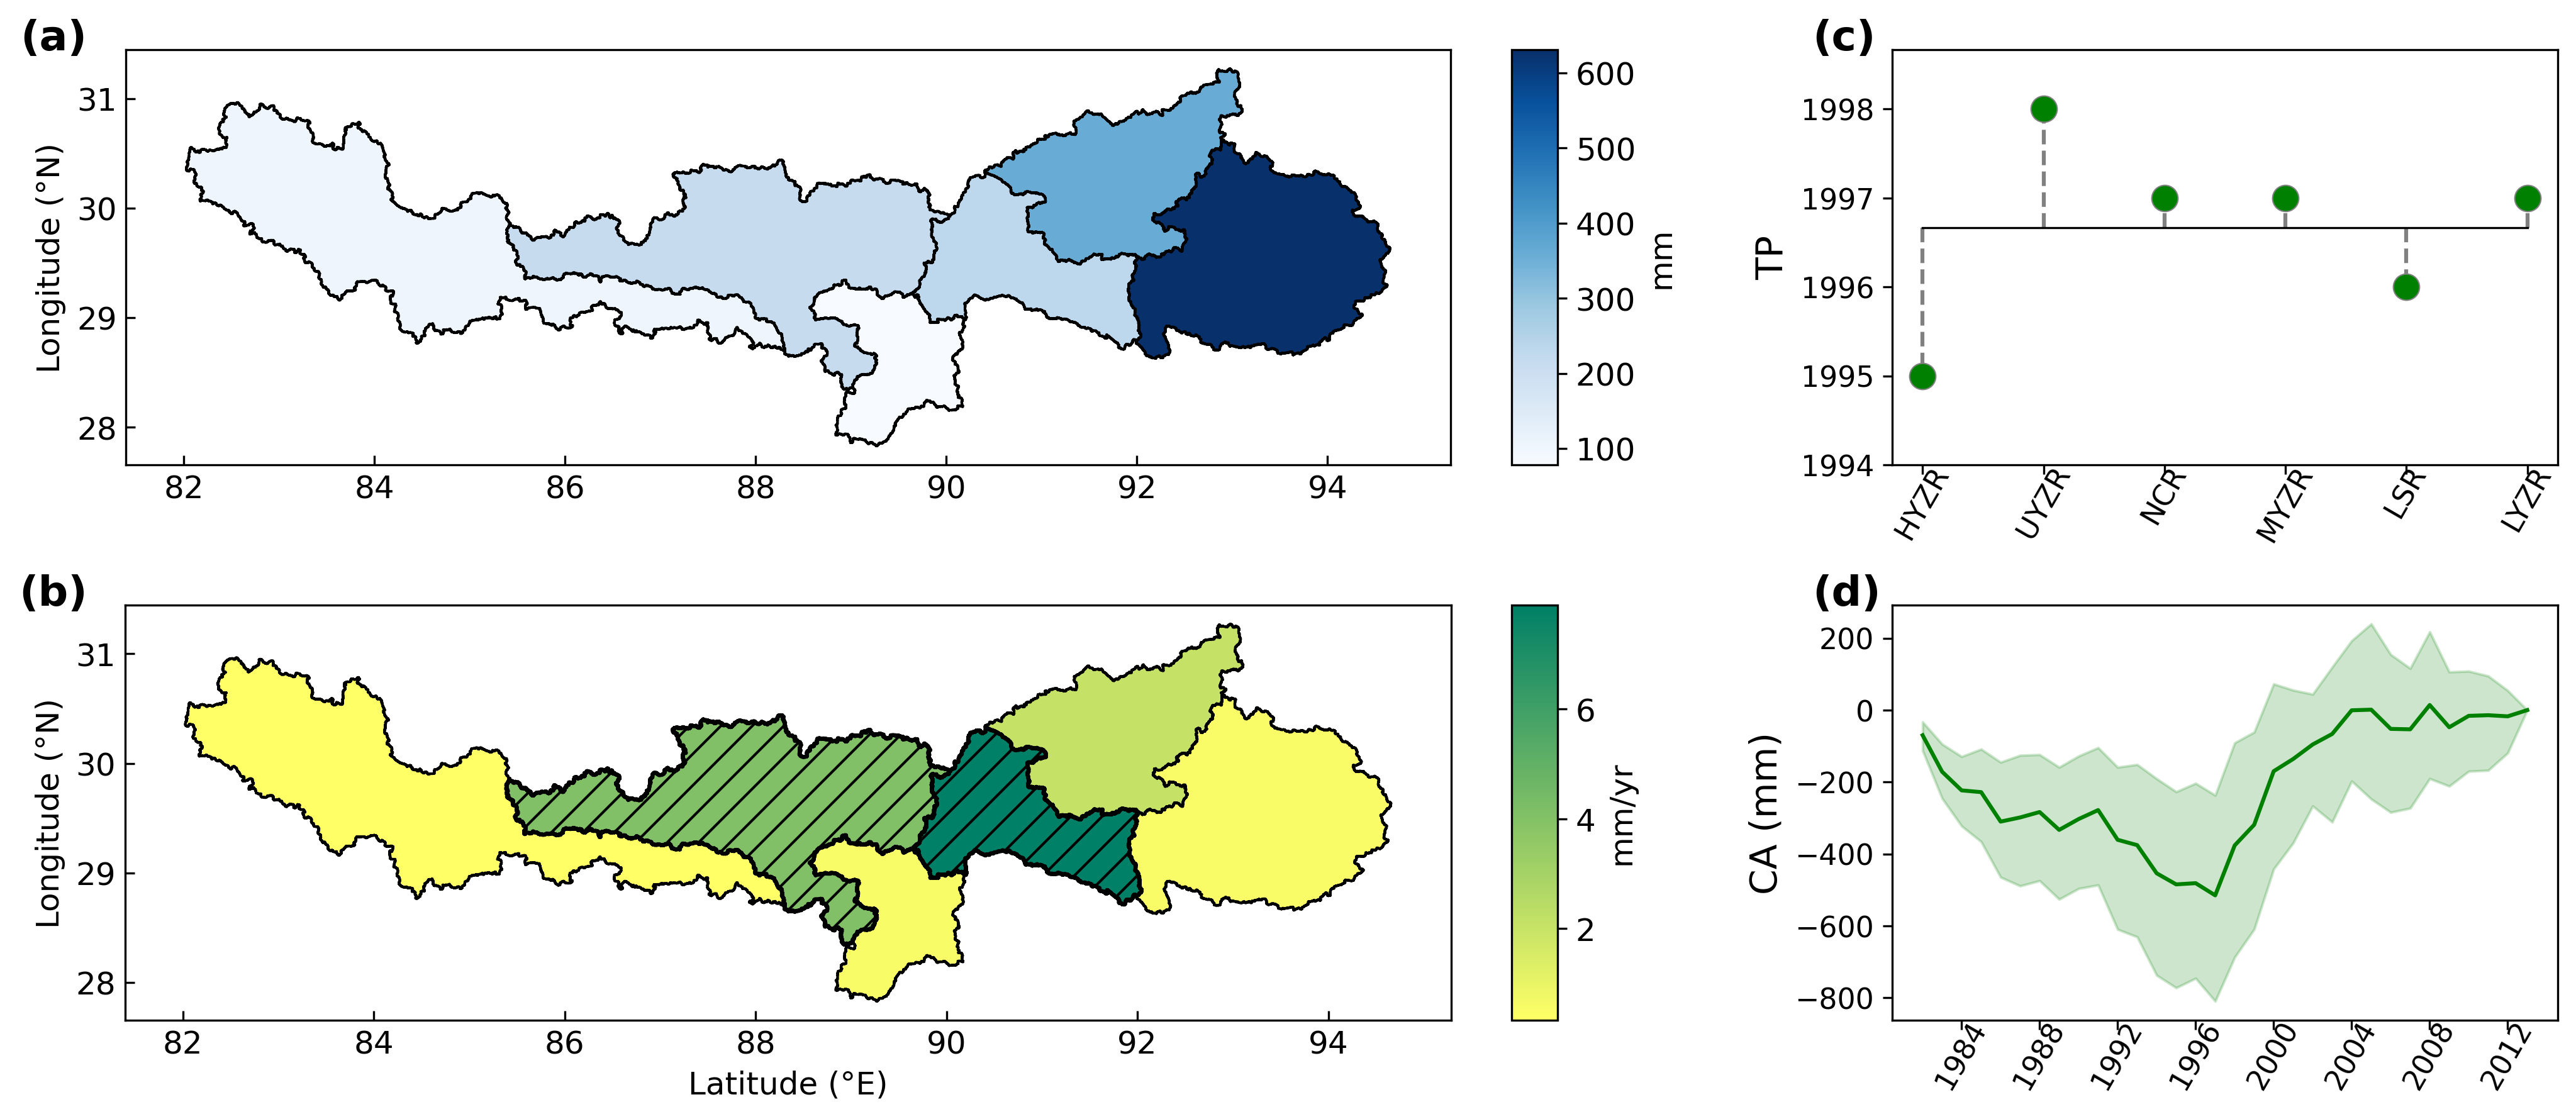
\includegraphics[width=12cm]{01-figures/Fig.2.png}
\caption{Long-term water yield changes over the six sub-basins, covering the entire UBR basin. (a) The mean annual values by
averaging water yield from 1982 to 2013. (b) The temporal variation trends detected by the Mann-Kendall Sen’s slope. The black
hatching represents statistically significant (p < 0.05) trends. (c) The turning points (TP) as detected by the Pettitt method. (d) The
cumulative water yield anomaly (CA) curve. The solid green line represents the ensemble expectation of the cumulative water yield
195 anomaly curves for the entire UBR basin (green shading).}
\label{fig:water-yield}
\end{figure*}

\subsection{Regime shifts in historical water yield}
Based on the TPs, we divided the study period from 1982 to 2013 into before and after TP periods, and analyzed the magnitude and direction of the WY changes over the entire UBR basin. Figure 3 shows that the WY increased from 9.5 to 130.9 mm, with high spatial variability. The slight increase observed in the HYZR and LYZR basins accounted for less than 10\% of the mean annual water yield before the TP. Nevertheless, a substantial increase in WY of 61.6\% and 80.5\% was found in the UYZR and MYZR basins, respectively. In addition, higher standard deviations were detected for WY after TP, suggesting more dramatic variability in the entire UBR basin in later years.

For the direction of the WY changes, we found that the change in WY was positive before the TP but became negative afterward in most sub-basins. A significant decreasing trend was detected after the TP in the UYZR, NCR, and LSR basins. In contrast, although the WY in the MYZR basin increased during two periods, the rate of increase had slowed, as the positive trend after the TP (3.64 mm yr$^{−1}$, p > 0.05) was less than that before the TP (8.95 mm yr$^{−1}$, p < 0.05). Overall, we found that regime shifts in the WY occurred in the late 1990s over the entire UBR basin; the magnitude of the WY changes generally increased, while the direction of the changes reversed or slowed.

\begin{figure*}[t]
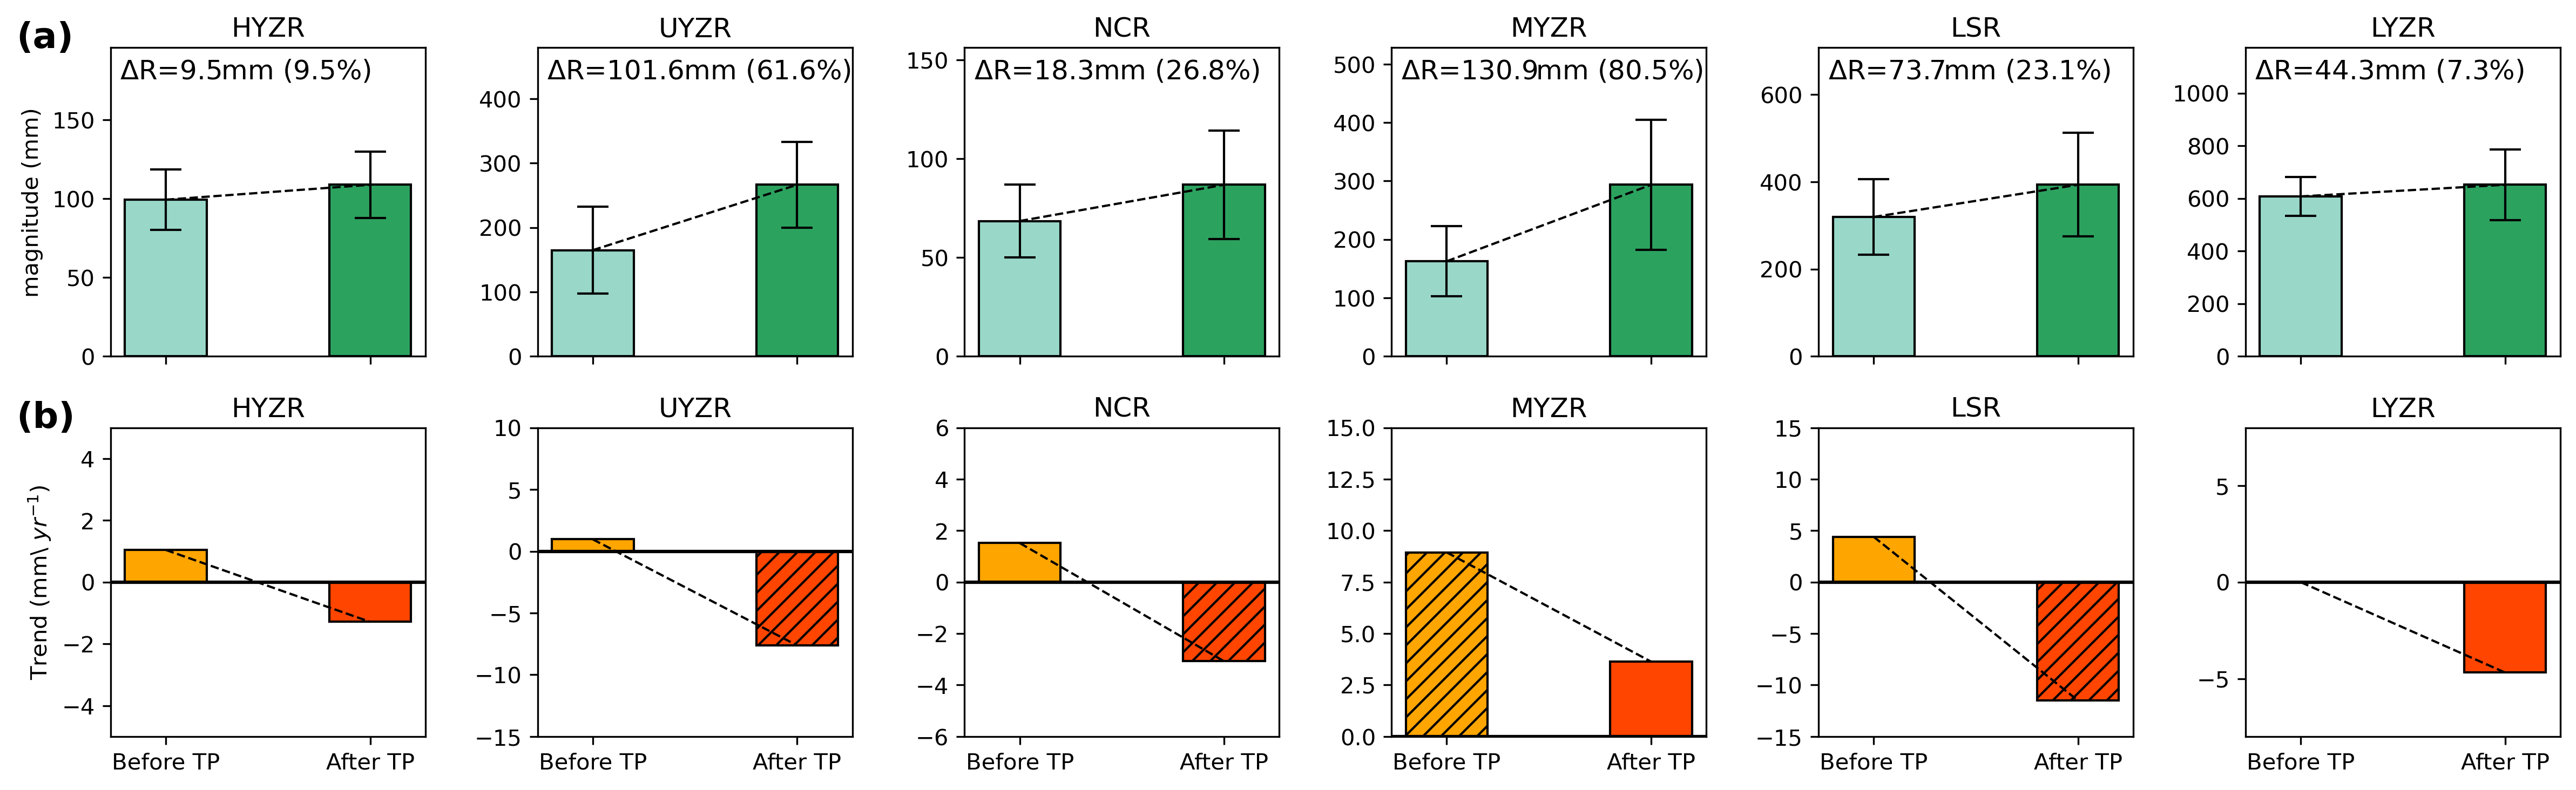
\includegraphics[width=12cm]{01-figures/Fig.3.png}
\caption{Water yield regime shifts over the entire UBR basin. (a) Magnitude of the water yield changes. The error bars represent the
standard deviation of the water yield before (light green) and after turning point (TP) (green). (b) Direction of the water yield changes.
The black hatching represents a statistically significant (p < 0.05) trend.}
\label{fig:magnitude-direction}
\end{figure*}

\subsection{Attribution analysis on magnitude increases in water yield}
As shown in Figure 4, we quantified the contributions from climate (eP), vegetation (LAI), and the cryosphere on the WY magnitude increases over the entire UBR basin. We found that the changes in the cryosphere contributed to over half of the magnitude increases in the HYZR, UYZR, NCR, and MYZR basins. However, climate played a more important role in the magnitude increase in the LSR and LYZR basins, with relative contributions of 55.4\% and 46.0\%, respectively. In contrast to the dominant roles of the climate and cryosphere, vegetation had a consistently positive contribution to the magnitude increases in WY over the entire UBR basin, although the relative contributions of 5.6\% in the HYZR basin and 19.9\% in the LYZR basin were much less than those from the changes in the climate and cryosphere.

The climate and cryosphere -- two important factors influencing the magnitude change in WY -- together contributed over 80\% to the magnitude increases over the entire UBR basin; however, they played both additive or offsetting roles (Figure 4), resulting in slight or substantial WY increases (Figure 3). For example, although the cryosphere change resulted in increases of 28.3 mm and 30.3 mm in the HYZR and NCR basins, the negative contributions from climate offset a considerable part of these increases resulting in the slight increase after the TP in these regions. Additionally, the positive contribution from climate offset the negative contribution from the cryosphere in the LSR and LYZR basins, which resulted in a similar slight increase in WY. However, the additive effects from the climate and cryosphere change lead to substantial increases in WY from 162.6 mm to 293.5 mm in the MYZR basin and from 164.9 mm or 266.5 mm in the UYZR basin.

\begin{figure*}[t]
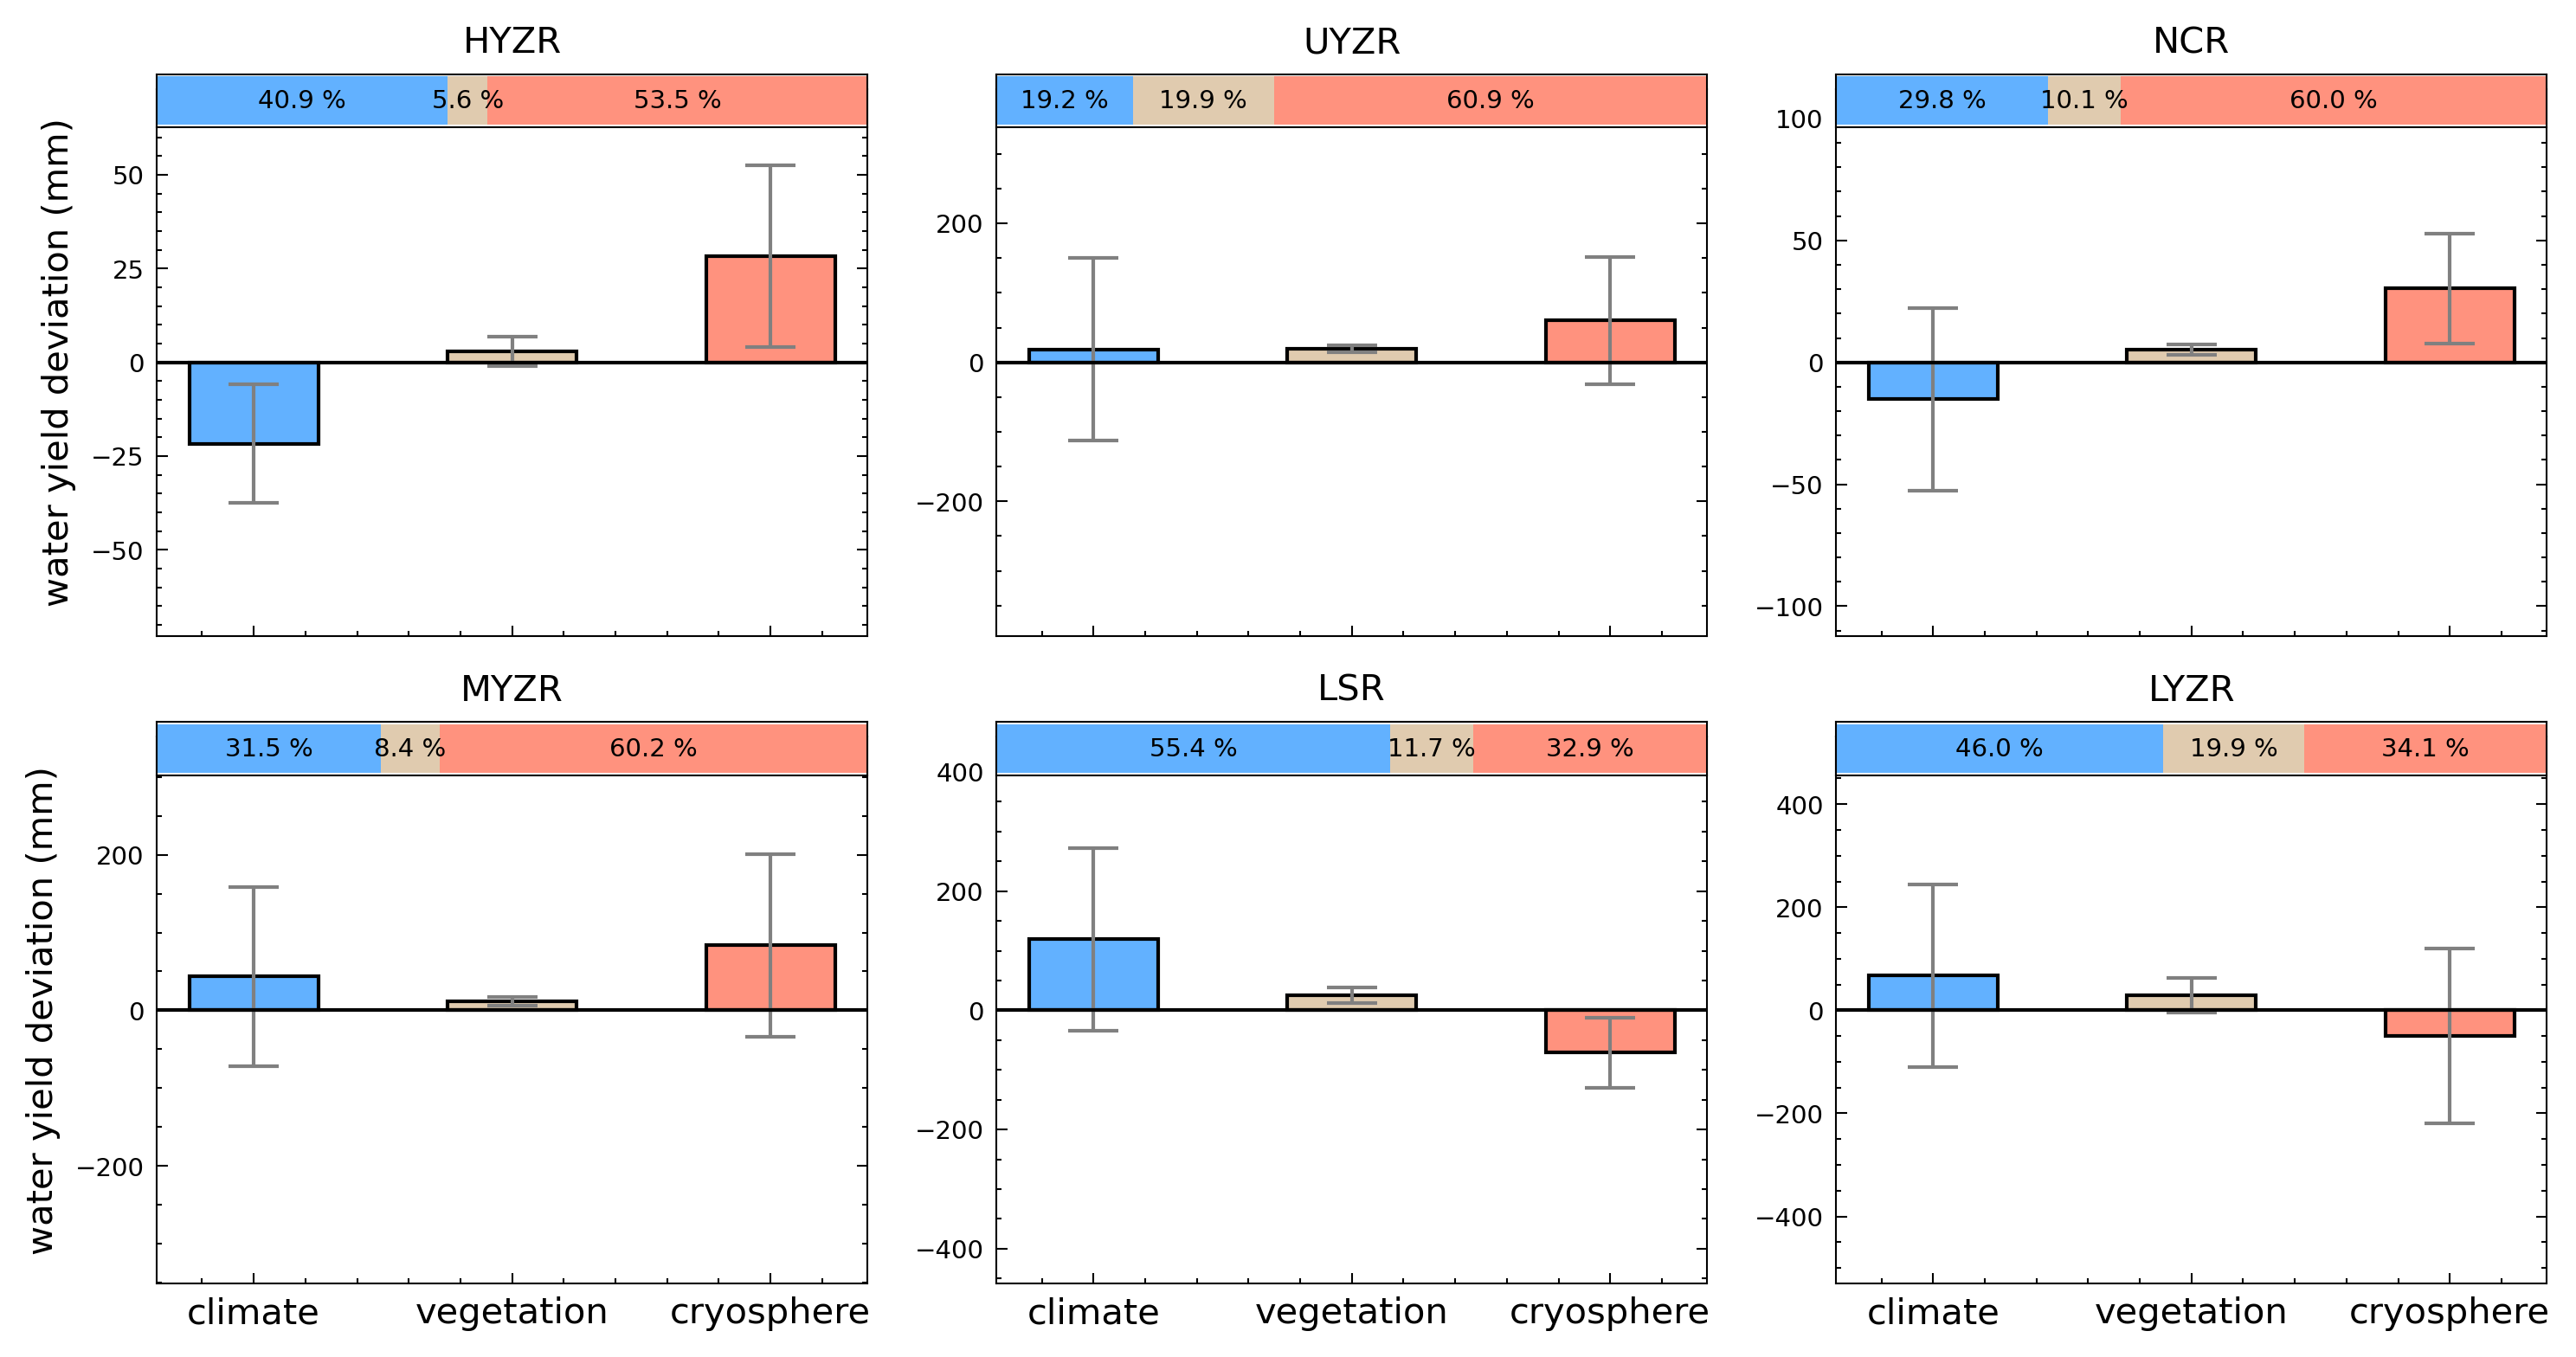
\includegraphics[width=12cm]{01-figures/Fig.4.png}
\caption{Attribution analysis of the magnitude increase in the water yield due to climate (blue bar), vegetation (tan bar), and the
240 cryosphere (red bar), and their relative contributions (the bar on the top) in each basin. The error bars represent the standard deviation of
the water yield changes caused by the various drivers (see Figure S2).}
\label{fig:magnitude-attribution}
\end{figure*}

\subsection{Attribution analysis on direction shifts in water yield}
In this study, Pearson’s correlation coefficient was applied to determine the role of the climate, vegetation, and cryosphere in the reversed or slowed WY trend after the TPs, as shown in Figure 3b. The climate played a dominant positive role in influencing the direction of the WY changes after the TP in most sub-basins (Figure 5), which was supported by correlations ranging from 0.41 (LYZR basin) to 0.93 (LSR basin). However, the changes in WY induced by the cryosphere instead determined the decreasing trend in WY over the HYZR basin (r = 0.76, p < 0.05). Compared to the significantly positive role of climate, however, cryosphere-induced changes in WY in the UYZR, NCR, and LSR basins exhibited a negative correlation with the decreased WY after the TP. This suggests that meltwater from the cryosphere alleviated the loss of water resources in these regions. In addition, this effect was also detected in the MYZR basin, and together with that of climate, contributed to the increasing trend in the WY in this sub-basin. Despite the weak contribution from vegetation compared to that of the other two drivers (Figure 4), its positive role in WY decline after the TPs was more apparent in the drier sub-basins (such as HYZR, UYZR, and NCR), whereas the correlation was negative in the humid LYZR basin.

\begin{figure*}[t]
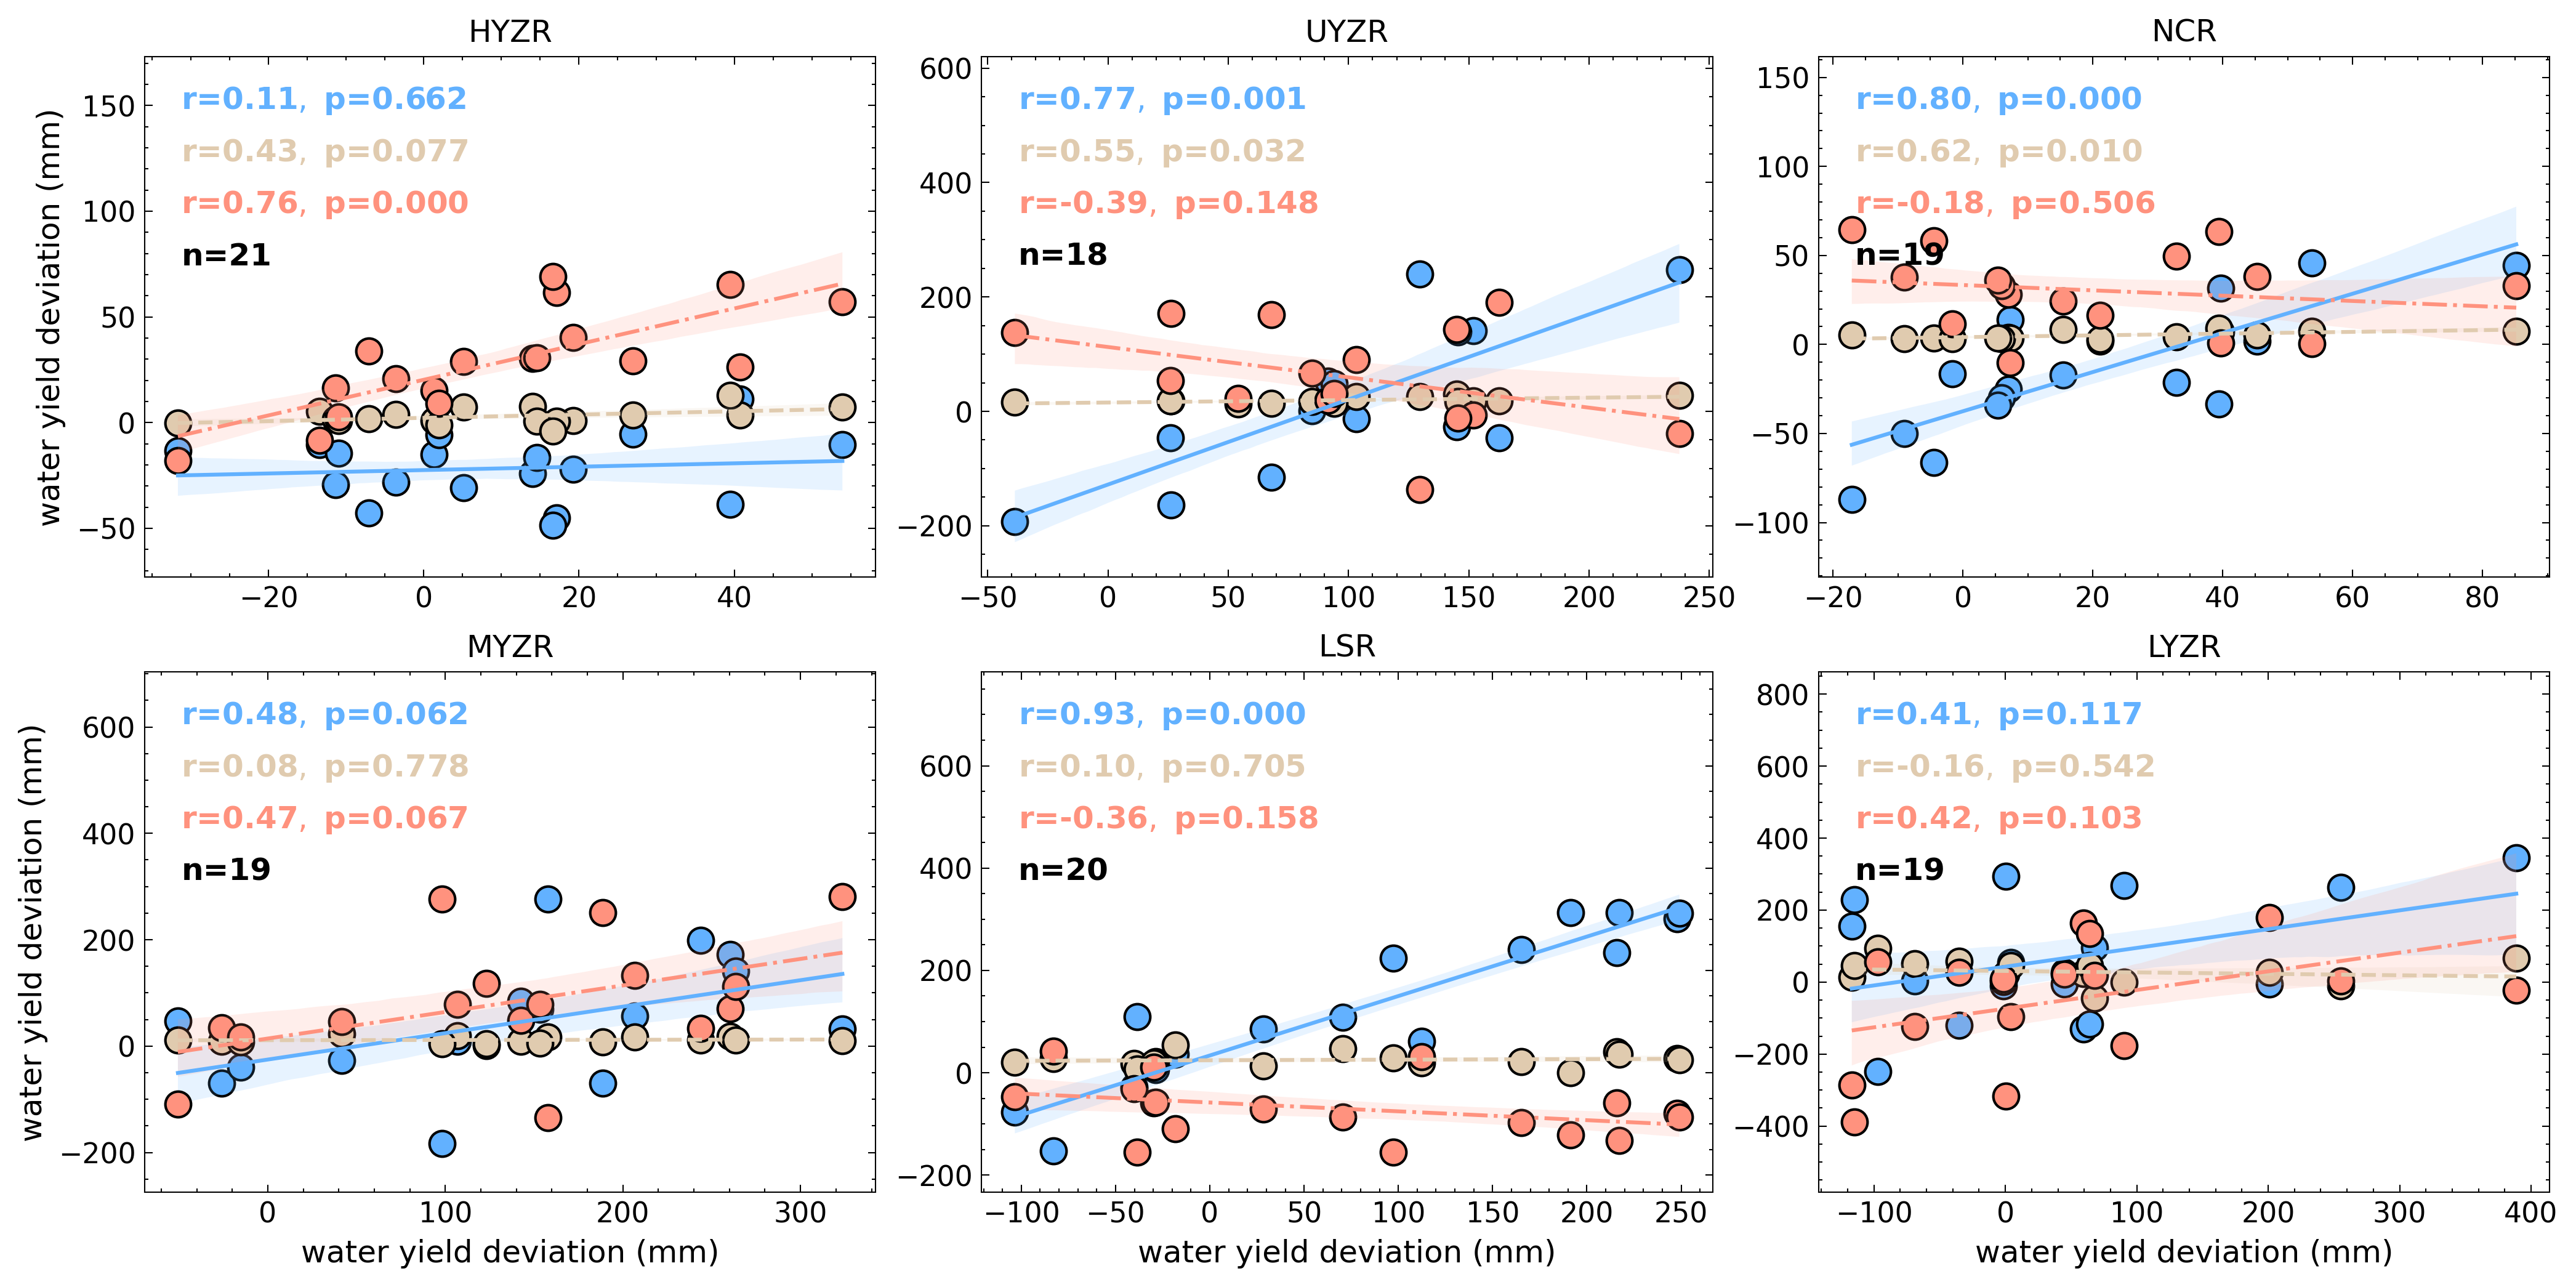
\includegraphics[width=12cm]{01-figures/Fig.5.png}
\caption{The relationship between the time-series of the total water yield deviation ($\Delta WY(t)$, x-axis) and its components (y-axis) induced
by climate ($\Delta WY_c(t)$, blue point), vegetation ($\Delta WY_v(t)$(t), tan point), and cryosphere ($\Delta WY_s(t)$, red point), respectively. The shading area
indicates the 95\% confidence interval of the fitting. n indicates the number of years after the TP, which was determined by the Pettitt
method (See Figure 2c and Table S2).}
\label{fig:direction-attribution}
\end{figure*}

\section{Discussion}
The changes in water yield can primarily be attributed to climate change and the cryosphere; nevertheless, they are affected by a complex variety of factors \citep{liu2020variability,harris2017geocryology}, such as vegetation, snow cover, permafrost, hydrology, and soil properties. 
Accurate monitoring of cryospheric processes is essential for understanding the changing composite interactions in alpine regions and predicting regional responses to climate warming \citep{yao2019recent}. Although some in situ observations have included more physical variables, such as soil moisture and temperature monitoring networks in Naqu and Pali \citep{chen2017evaluation}
and observations of snow and glacial melt runoff in glacier-fed basins \citep{zhang2016modeling}, there remain large unassessed areas in the UBR basin.
The harsh climate and environmental conditions in these regions remain quite challenging to accurate cryosphere-hydrological modeling. In this study, with the support of the Hydrology and Water Resources Survey Bureau of the Tibet Autonomous Region, we collected long-term runoff-gauge data throughout the UBR, examined historical water yield changes, and provided a useful alternative statistical method to physical modeling approaches that can be applied to large-scale alpine river basins to quickly partition the effects of climatic and cryospheric changes on the hydrological regime. Nevertheless, further numerical modeling tools with coupled cryospheric and hydrospheric processes and comprehensive observational data \citep[e.g.,]{wang2017development} should be developed to better physically and comprehensively understand the mechanisms of the runoff variations in the UBR basin.

Previous studies have demonstrated an increasing trend in WY over the LSR \citep{linhess2020}, LYZR \citep{zhangech2011}, and UBR basins \citep{li2021vegetation}. In this study, we provided further evidence of the long-term trends in WY changes in the above regions, and, furthermore, conducted trend analysis for other regions that have received less attention in the existing literature. Our results comprehensively indicated a general increase in WY (Figure 2a) over the entire UBR basin. Furthermore, we extended the duration of the runoff observations to 2013 and found that regime shifts in WY occurred during the late 1990s over the entire UBR basin. Moreover, the magnitude of WY increased (Figure 3a), but the direction of WY reversed or slowed after the TPs (Figure 3b). To the best of our knowledge, these regime shifts in the WY have not been reported in previous studies.

Our results indicated that the climate and cryosphere were important factors for magnitude increases in WY throughout the UBR basin, but their relative contribution varies across regions. Climate explained a greater increase in WY in downstream regions, while cryospheric changes were more important in upstream regions (Figure 4); this matches the relative importance of meltwater from the cryosphere to streamflow (Figure S4). According to \citet{biemans2019importance}, meltwater from the cryosphere is the most important water source in the upper regions of the Indo-Gangetic Plain, supplying over 40\% of the total WY upstream but less than 30\% downstream. The effect of vegetation on changes on WY was much less than that of the climate and cryosphere (Figure 4 and Figure S2). Additionally, offsetting or additive effects from climate and cryosphere changes were detected in this study (Figure 4), which led to either slight or substantial increase in WY in each region of the UBR basin (Figure 3a). The additive effect is beneficial for mitigating drought, but it could exacerbate the flood risks due to increased precipitation and accelerated melting of the cryosphere in the future \citep{Immerzeel2013}. More importantly, the combined effects often hinder the roles of each driver in hydrological changes, which should be considered when designing water management strategies and ecological restoration engineering \citep{wei2018,zhang2021deforestation}.

Although climate and cryosphere together contributed to the magnitude increases in WY throughout the UBR basin, climate remained the most important factor controlling the declining WY in most regions (Figure 5). Simultaneously, significant cryosphere changes due to global warming influenced the direction of the WY changes, which is supported by glacier retractation \citep{yao2010glacial} and several modeling studies \citep{lutz2014consistent,Zhang2020VariationOM, wang2021tp, wang2021vanishing}. Similarly, our study indicated that meltwater from cryospheric changes has the potential to alleviate reduced water resources in most regions (Figure 3b). However, in the HYZR basin, the decline in cryosphere-induced WY became a more important driver of the decreasing WY trend after the TP, which was inferred from the strong positive correlation (r = 0.76, p < 0.05, Figure 5). The meltwater from snow and glaciers in the cryosphere accounted for over 60\% of the streamflow in the HYZR basin \citep{biemans2019importance} and was critical for regional ecology; however, our statistical results suggested a decreasing supply from the cryosphere after the TP in the HYZR basin, which could be important for ecological restoration in river sources and emphasizes more explicit physical-based cryosphere--hydrology modeling.

Effective precipitation, an integrated climatic index that was generated by subtracting the actual evapotranspiration from the precipitation, was used in the DMC method. As shown in Figure S3, the mean annual WY of all six sub-basins showed a consistently linear relationship with the corresponding mean annual precipitation, further proving the dominant role of precipitation in the spatial and temporal characteristics of the WY throughout the UBR basin. In addition, \citet{wei2018} and \citet{zheng2009responses} conducted attribution analyses of the streamflow caused by climate and land surface changes in large-scale river basins with mountains and diverse vegetation; they indicated that streamflow variation and climate variability show a linear relationship, which provides solid evidence for the assumption of a linear relationship between the WY variation and effective precipitation in the present study. Furthermore, the results prove that the effects of climate variability could be successfully separated to present a clearer picture of the cumulative and annual effects of the cryosphere and vegetation changes on the WY in the UBR basin.

\conclusions  %% \conclusions[modified heading if necessary]
In this study, regime shifts in WY were detected during the late 1990s over the UBR basin. The magnitude of the WY generally increased, but its direction reversed or slowed. We used the DMC method to assess the effects of the climate, vegetation, and cryosphere on the WY and found that the changes in the climate and cryosphere had either an offsetting or additive effect, which caused either a slight or substantial increase in the WY, whereas the role of vegetation was much smaller. Furthermore, the declining or slowing WY after the TPs was mainly driven by climate in most regions, and notably, meltwater from the cryosphere had the potential to alleviate reduced water resources. These findings suggest that the combined effects of the climate and cryosphere should be considered in the sustainable development of water resources and ecosystems, especially the co-benefits in upstream and downstream regions.

%% The following commands are for the statements about the availability of data sets and/or software code corresponding to the manuscript.
%% It is strongly recommended to make use of these sections in case data sets and/or software code have been part of your research the article is based on.

%\codeavailability{TEXT} %% use this section when having only software code available

\dataavailability{The datasets generated for this study are available on request to the corresponding author.} %% use this section when having only data sets available

%\codedataavailability{TEXT} %% use this section when having data sets and software code available

%\sampleavailability{TEXT} %% use this section when having geoscientific samples available

%\videosupplement{TEXT} %% use this section when having video supplements available

%\noappendix       %% use this to mark the end of the appendix section. Otherwise the figures might be numbered incorrectly (e.g. 10 instead of 1).
%\appendix
%\section{}    %% Appendix A

%\subsection{}     %% Appendix A1, A2, etc.

%% Regarding figures and tables in appendices, the following two options are possible depending on your general handling of figures and tables in the manuscript environment:

%% Option 1: If you sorted all figures and tables into the sections of the text, please also sort the appendix figures and appendix tables into the respective appendix sections.
%% They will be correctly named automatically.

%% Option 2: If you put all figures after the reference list, please insert appendix tables and figures after the normal tables and figures.
%% To rename them correctly to A1, A2, etc., please add the following commands in front of them:

%\appendixfigures  %% needs to be added in front of appendix figures
%\appendixtables   %% needs to be added in front of appendix tables
%% Please add \clearpage between each table and/or figure. Further guidelines on figures and tables can be found below.

\authorcontribution{HL: conceptualisation, data curation, formal analysis, methodology, writing--original draft, writing -- review and editing. LL: conceptualisation, formal analysis, methodology, writing -- review and editing, funding acquisition. BYS: data curation, methodology. LW: supervision, writing -- review and editing. AK: validation, writing -- review and editing. FZ\&DFL: software, validation. XXW: visualization. WFL\&XPL: Writing -- review \& editing. ZXX: supervision, resources.} %% this section is mandatory

\competinginterests{The contact author has declared that neither they nor their co-authors have any competing interests.} %% this section is mandatory even if you declare that no competing interests are present

%\disclaimer{TEXT} %% optional section

\begin{acknowledgements}
This work was jointly supported by the National Natural Science Foundation of China (Grant No. 51961145104, 52079138, and 91647202), the 2115 Talent Development Program of China Agricultural University (00109019), and the China Scholarship Council (Grant No. 202006350051). Hao Li thanks the China Scholarship Council (CSC) for providing financial support to pursue his PhD in Belgium.
\end{acknowledgements}


%% REFERENCES
\bibliographystyle{copernicus}
\bibliography{reference.bib}


\end{document}
